
\documentclass[preprint,12pt]{elsarticle}

\usepackage[spanish]{babel}
\usepackage{amssymb}
\usepackage{graphicx}
\usepackage{lineno}
\usepackage[utf8]{inputenc}
\usepackage{url}
\usepackage{natbib} 
\usepackage{amsmath} 
\usepackage{amssymb} 

\begin{document}
	
	\begin{frontmatter} 

		\title{\huge DevOps en Base de Datos}
		
		\author{Estrella Palacios, Katherine Lizbeth              	(2016056193))}
		\author{Gonzales Cave, Angel Gabriel              	(xxxxxxxxxx))} %%cambiar
		\author{Huichi Contreras, Franklin Carlos         	(2016054948))} 
		\author{Huillca Umpiri, Willian Arturo             		(xxxxxxxxxx))} %%cambiar 
		\address{Escuela Profesional de Ingeniería de Sistemas}
		\address{Universidad Privada de Tacna}
		\address{Tacna, Perú}
		
%% ABSTRACT --------------------------------------------------------------------------------------------------------------------

		\begin{abstract}
		
Devops is described as a cooperative and productive relationship between development teams and operating teams. That is why DevOps manages to establish an effective relationship of efficiency, collaboration and development strategies among employees.
DevOps also adopts new development methodologies such as agile development, operations, quality control and implementation in order to create integration and collaboration between the two departments.
In conclusion, communication and collaboration between the departments of developers and operations make this methodology the best option to resort to an orderly and well-structured work model.

		\end{abstract}

%% ----------------------------------------------------------------------------------------------------------------------------------

	\end{frontmatter}

%% RESUMEN ---------------------------------------------------------------------------------------------------------------------

\section{Resumen}

Devops es describido como una relación cooperativa y productiva entre los equipos de desarrollo y los equipos de operación. Es por ello que DevOps logra establecer una relación eficaz, de eficiencia, colaboración y estrategias de desarrollo entre los colaboradores.
DevOps también adopta nuevas metodologías de desarrollo como el desarrollo ágil, operaciones, control de calidad e implementación con el fin de crear integración y colaboración entre los dos departamentos.
En conclusión, la comunicación y colaboración entre los departamentos de desarrolladores y operaciones hacen de esta metodología la mejor opción para recurrir a un modelo de trabajo ordenado y bien estructurado.

%% ----------------------------------------------------------------------------------------------------------------------------------


%% INTRODUCION ----------------------------------------------------------------------------------------------------------------

\section{Introducción}  %%MODIFICAR CONTENIDO, PERO CONSERVAR CANTIDAD DE LINEAS DEL PÁRRAFO

Con la llegada de las metodologías ágiles de desarrollo y las necesidades de realizar integración y entrega continua (CI, continuous integration y CD,
continuous delivery) aparece una nueva corriente organizativa llamada DevOps, que, en resumidas cuentas pretende aunar en un único equipo a
perfiles muy separados en organizaciones más tradicionales como puedan ser los desarrolladores y los equipos de operaciones, todo ello con el objetivo final
de realizar despliegues en entornos productivos de forma más regular. Haciendo nuevas entregas del software de una forma regular (semanalmente, diariamente o, incluso, varias veces al día) se consigue dotar al proceso del paso a producción de más seguridad o estabilidad y más eficiencia. Cuanto
más regularmente se haga una tarea, en este caso un despliegue en producción, menos «doloroso» será. Para ello se requiere un nivel muy alto en
la automatización de los procesos de compilación, empaquetado, pruebas, despliegues, smoke tests, etc.

%% ----------------------------------------------------------------------------------------------------------------------------------


%% MARCO TEÓRICO ------------------------------------------------------------------------------------------------------------

\section{Marco Teórico}

%% PRIMERA SUBSECCION 

\subsection {\textbf{DevOps}}

\subsubsection{\textbf{Definición}}

DevOps fue acuñado en 2009 por Patrick Debois, que se ha convertido desde entonces en uno de los gurús dentro de la comunidad. El término se conforma de combinar las palabras "desarrollo" y "operaciones, del inglés "Development \& Operations", y puede servir como punto de partida para entender qué significa exactamente el término DevOps. Esta nueva cultura no es un proceso, una tecnología concreta o un estándar, sino un conjunto de técnicas, pensamientos, y modelos de trabajo. También se utiliza el término "movimiento DevOps" cuando se habla de temas acerca de la adopción de nuevos ratios e indicadores y tendencias de futuro y "entorno DevOps" para referirse a la estrategia organizativa que sugiere la cultura DevOps. \cite{Walls2013} 

DevOps representa un cambio en la cultura de TI, centrándose en la entrega rápida de servicios de TI a través de la adopción de prácticas ágiles y esbeltas en el contexto de un enfoque orientado al sistema. DevOps hace hincapié en las personas (y la cultura) y busca mejorar la colaboración entre las operaciones y los equipos de desarrollo. Las implementaciones de DevOps utilizan tecnología, especialmente herramientas de automatización que pueden aprovechar una infraestructura cada vez más programable y dinámica desde una perspectiva del ciclo de vida  \cite{Gartner} 

\subsubsection{\textbf{Beneficios}}

En una encuesta reciente, realizada a 1.770 altos ejecutivos de TI a nivel mundial, por el instituto Technologies y el Coleman Parks Research, han llegado a la conclusión de que existen al menos 8 beneficios que se pueden obtener de la implementación de las DevOps en el ámbito empresarial. 
\\Los resultados a los que estas dos empresas llegaron luego de su estudio, son los siguientes: \cite{TicNews2017}   
\begin{itemize}

\item Más plazas de trabajo
%%Según los encuestados, el uso de las DevOps ha tenido un impacto positivo en el número de contrataciones y, en la cantidad de personas que se mantenían en los puestos de trabajo.

\item La buena experiencia del cliente
%%Aunque a menudo es el marketing el que influye positivamente en la experiencia del usuario, se ha demostrado que la tecnología juega un papel clave en este aspecto, muy probablemente, debido a que somos una sociedad cada vez más familiarizada y ávida de conocimientos tecnológicos.

\item Un cliente feliz es una empresa exitosa
%%Para estimar el grado de satisfacción del cliente, se valieron de una encuesta métrica conocida como NPS (Net Promoter Score), en la que se le hace una serie de preguntas el encuestado, que debe dar su respuesta en base a una escala del 1 al 10.

\item Empleados más productivos
%%No sólo los clientes se sienten más a gusto, sino que, con una mayor integración y conocimiento de las diferentes áreas de trabajo de la empresa, los empleados se sienten más involucrados en su puesto de trabajo y, por consiguiente, su desempeño es mayor.

\item Calidad de la aplicación
%%Por lo general, para determinar la calidad de una aplicación, se evalúan el número de defectos que ésta posee. Luego del estudio, se llegó a la conclusión de que la incorporación de las DevOps disminuye en al menos un 41\% estas fallas en el sistema.

\item Eficiencia de los procesos
%%Una de las principales funciones de las DevOps es mejorar la calidad de los procesos de la empresa, por lo que no es de extrañar que ocurra una mejoría significativa en este aspecto.

\item El crecimiento de nuevos negocios
%%Al aumentar la eficacia de los procesos de las empresas, aunado al ahorro significativo de costos, muchas compañías han sido capaces de emprender nuevos negocios, aprovechando el espacio libre que ha quedado.

\item Reducción de costos en las TI
%%Según las encuestas, las empresas que adoptaron las DevOps experimentaron una reducción en los costos. Esto se debe en gran medida al aumento de la eficiencia y productividad. 

\end{itemize}

\subsubsection{\textbf{Principios}}

DevOps maneja principios que son parte de la estructura colaborativa y son utilizados en toda la etapa de desarrollo y despliegue de aplicaciones. \\Los principios en los que se desenvuelve DevOps son los siguientes:  \cite{Humble2011}   \cite{Huttermann2012}   

%%Según Martin Fowler, entrega continua y despliegue continuo son términos similares y crean cierta confusión en algunos autores. Él define la diferencia como una decisión de negocio sobre la frecuencia de despliegue en producción. Entrega continua se trata de mantener la aplicación en un estado en el que siempre es capaz de desplegarse en producción. Despliegue Continuo consiste en desplegar todos los cambios en producción, todos los días o con mayor frecuencia. (http://martinfowler.com/delivery.html)%%

\begin{itemize}

\item \textbf{Integración Continua}
La Integración Continua es la forma en la que el equipo de desarrollo de software integra su trabajo parcial o total, en un determinado tiempo establecido por el equipo de trabajo. Requiere de herramientas de automatización que son únicas para todo el equipo de desarrolladores. Estas herramientas ayudan a integrar en forma continua partes de código que son validados por pruebas automáticas, lo cual vuelve más eficiente el trabajo del equipo de desarrollo, ya que permite detectar fallos en etapas tempranas del ciclo de desarrollo.
La Integración continua de cada uno de los integrantes del equipo va a favorecer en los tiempos y calidad del producto.La automatización de la integración continua ayuda a descubrir errores, debido a las continuas pruebas de unidad automatizadas. 
%% La Integración Continua ayuda a establecer en forma ordenada los avances que pueda tener la iteración de las tareas que se están automatizando. 
\begin{figure}[htb]
	\begin{center}
		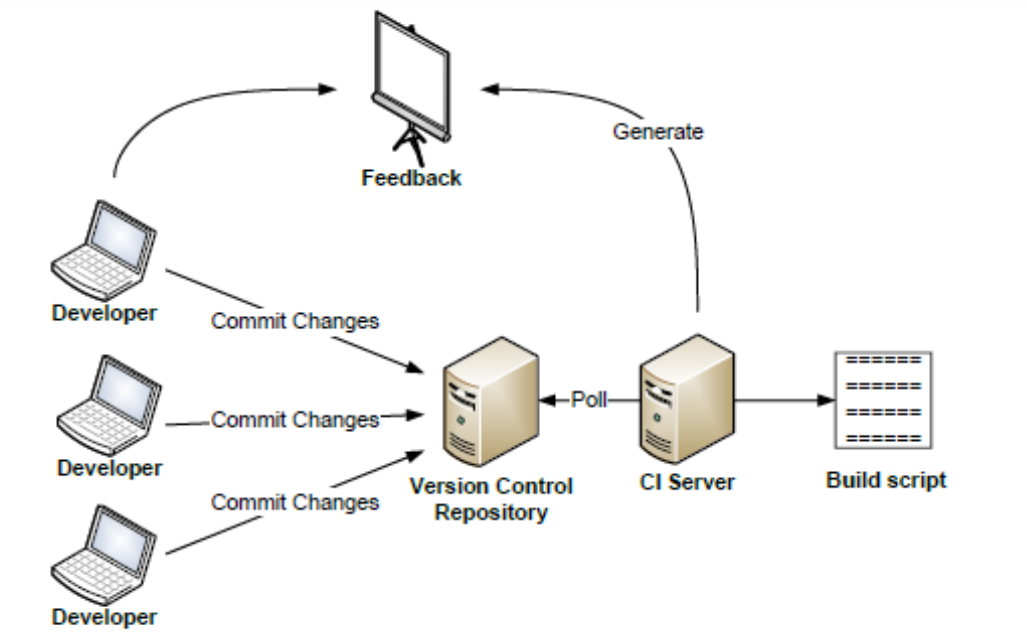
\includegraphics[width=8cm]{./IMAGENES/proceso_integracion_continua} 
		\caption{Proceso de Integración Continua}
	\end{center}
\end{figure}


\item \textbf{Entrega Continua}
Una vez lograda la integración, se debe continuar con el ciclo para realizar el testing que, si es satisfactorio, permita que la aplicación sea desplegada.
En esta etapa se implementan todos los cambios en el código y se somete a un proceso de pruebas estandarizado con el fin de generar un producto que pueda ser pasado a producción.
%%La entrega continua requiere una aprobación manual. Los periodos de tiempo para lograr entregas continuas depende que la organización cuente con el equipo de desarrollo y operaciones adecuado. De esta manera se pueden presentar versiones candidatas en tiempos mínimos. 
\begin{figure}[htb]
	\begin{center}
		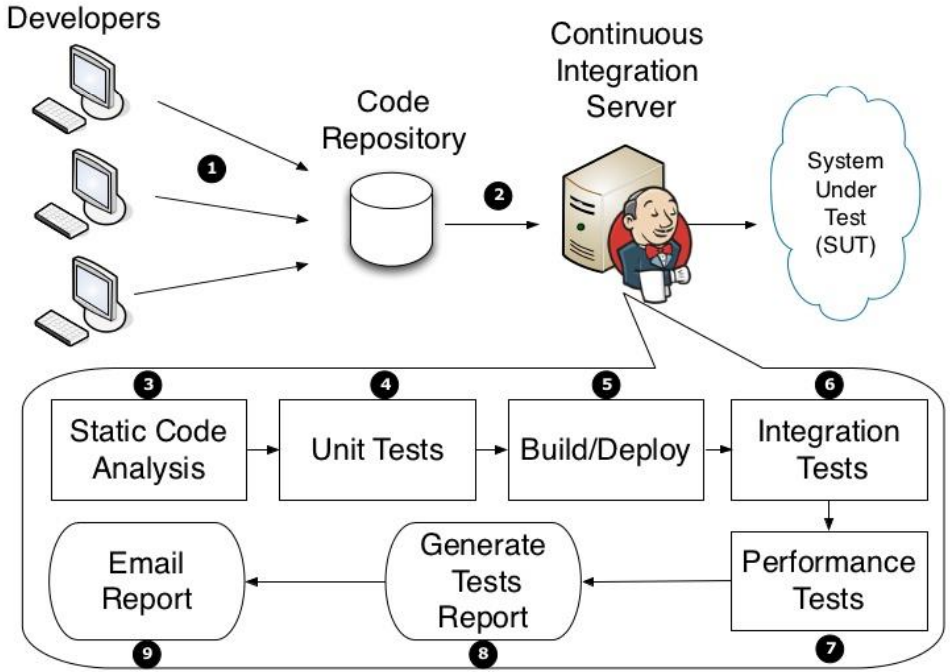
\includegraphics[width=7cm]{./IMAGENES/proceso_entrega_continua} 
		\caption{Proceso de Entrega Continua}
	\end{center}
\end{figure}


\item \textbf{Despliegue Continuo}
El despliegue continuo es una práctica que permite llevar los resultados de un proceso de desarrollo a un entorno similar al de producción donde las pruebas funcionales puedan darse a escala completa. El objetivo es detectar problemas en producción lo más rápido posible.
%% Es el momento temprano en que el usuario interactúa con la aplicación, revisa sus requerimientos y se puede volver atrás en el desarrollo.
%%El Despliegue Continuo exige una configuración del ambiente de trabajo, que permita un funcionamiento efectivo de las versiones candidatas por parte de los usuarios. Se empieza con una pre-configuración durante todo el proceso de desarrollo y una configuración final antes que se termine la versión candidata.
%%La entrega continua requiere de una aprobación manual previo a su paso a producción; en el despliegue continuo el paso a producción se realiza de forma automática cuando se han satisfecho todos los criterios definidos.
%%El Despliegue Continuo visualiza tempranamente los fallos que puedan existir en la aplicación.
%%Realizando Despliegues Continuos, se logra entregar productos al usuario que pueden ser diarios o semanales, y así analizar fallos que van a ser detectados en forma temprana, debido al poco código que hay que revisar.
\begin{figure}[htb]
	\begin{center}
		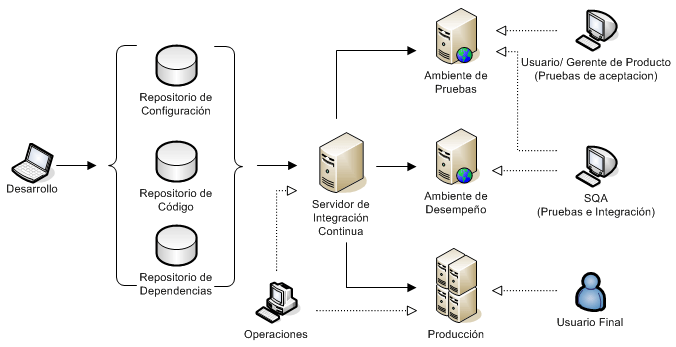
\includegraphics[width=8.5cm]{./IMAGENES/proceso_despliegue_continuo} 
		\caption{Proceso de Despliegue Continuo}
	\end{center}
\end{figure}


\end{itemize}

\subsubsection{\textbf{Ámbito de aplicación de DevOps}}
La mayoría de estas empresas organizan la estructura en dos grandes ámbitos, el de desarrollo de software y el de operaciones. A su vez, estos dos ámbitos tienen sus propios departamentos, los cuales pueden variar en función de las necesidades de cada empresa. Algunos de ellos pueden aparecer fusionados, o en
ocasiones prescindir de ellos dado que el volumen de negocio no lo requiere. Un ejemplo de los distintos departamentos que puede haber en una empresa es que se muestra en la siguiente figura: \cite{Jimenez2016}   
\begin{figure}[htb]
	\begin{center}
		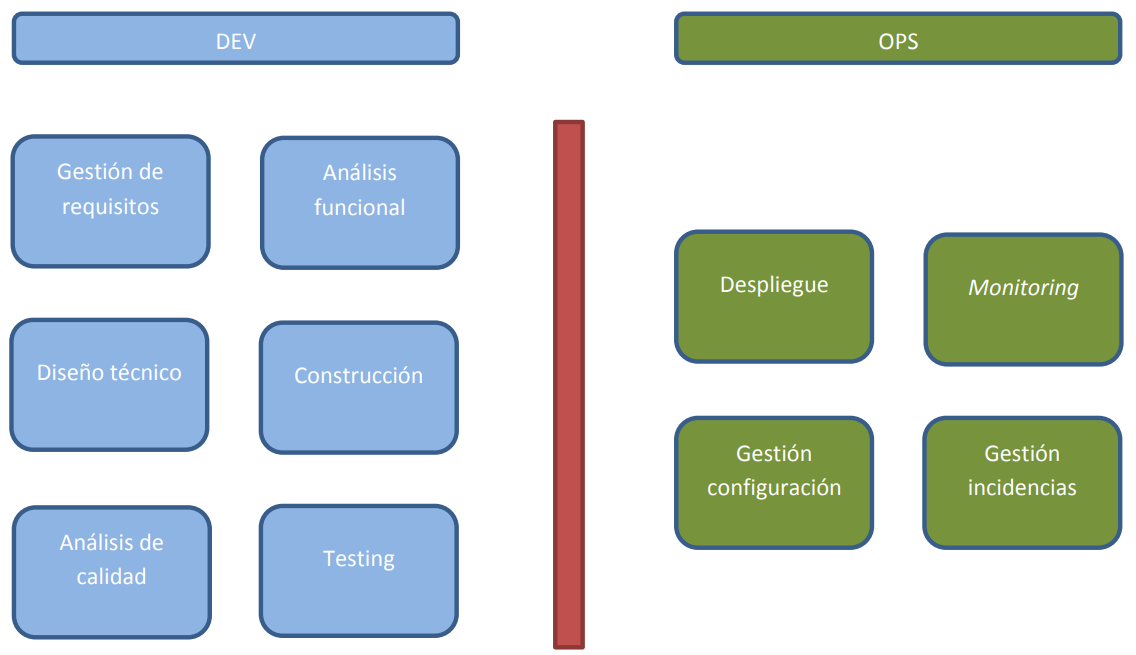
\includegraphics[width=11cm]{./IMAGENES/aplicacion_devops} 
		\caption{Ciclo de Vida del DevOps}
	\end{center}
\end{figure}


\subsubsection{\textbf{Ciclo de Vida y Herramientas de DevOps}}
Una cadena de herramientas es un conjunto de herramientas de programación que se pueden utilizar para llevar a cabo una tarea compleja de desarrollo de software o para crear un producto de software, que comúnmente es algún otro programa informático o un conjunto de programas relacionados. En el campo DevOps, son recursos útiles en la entrega, desarrollo y administración de aplicaciones durante el ciclo de vida de desarrollo de software, según lo coordinado mediante el uso de una organización que utiliza las prácticas DevOps.\cite{Perez2018} 
El ciclo de vida de DevOps consta de las siguientes etapas: Planificar, Crear, Verificar, empaquetar, liberar, configurar y monitorear. \cite{Platzi2019}   
\begin{figure}[htb]
	\begin{center}
		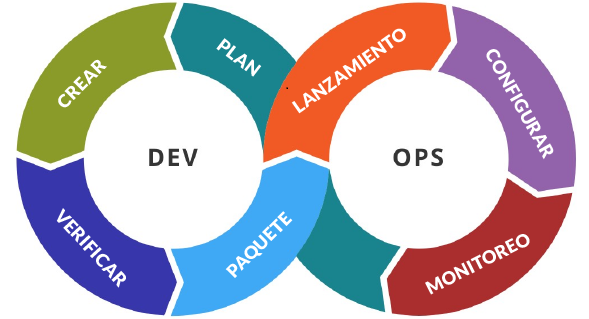
\includegraphics[width=8.5cm]{./IMAGENES/ciclo_devops} 
		\caption{Ciclo de Vida de DevOps}
	\end{center}
\end{figure}

\begin{itemize}
\item \textbf{Plan}
Sin importar la metodología que uses como Waterfall o Agile, en esta primera etapa definimos las labores del equipo, los requerimientos necesarios a implementar en la plataforma o producto.
Podemos hacer usos de herramientas como issues para hacer un monitoreo de nuestro progreso, así como boards como Trello o Asana.

\item \textbf{Create}
Empezamos a escribir el código que necesitamos para resolver los problemas que planteamos en el paso anterior.
Todo este código puede estar almacenado en un solo lugar como un repositorio de Github o Gitlab para hacer uso de herramientas proporcionadas por estas páginas y por git en general como branchs, tags y mucho más.

\item \textbf{Verify}
Como somos desarrolladores increíbles, hemos escritos diferentes pruebas de software para disminuir la cantidad de bugs que podemos agregar a nuestro producto una vez estemos en producción, también es una manera de descubrir errores. Estas pruebas son definidas con antelación.
Se pueden usar varias herramientas de Continuous Integration como TravisCI, CircleCI o Jenkins

\item \textbf{Package}
Empaquetamos nuestro código para correr en una infraestructura determinada. Esto puede hacerse incluso desde la etapa de creación donde escribimos nuestro código de una forma empaquetada y lista para que sea llevada a producción para no tener complicaciones y dolores de cabeza en el futuro.
Es muy común realizarlo en contenedores de Docker.

\item \textbf{Release}
Automatizamos el proceso de enviar el código a producción, liberar una nueva versión de nuestro producto cada que construyamos un feature nuevo o resolvamos un bug mientras haya pasado por las etapas anteriores.
No es más que una nueva versión de nuestro código disponible para hacerlo de manera manual o automática.

\item \textbf{Monitor}
Necesitamos revisar las métricas necesarias de cómo nuestro código está funcionando, qué tipo de performance ocurre en los dispositivos de nuestros clientes para tratar de optimizar siempre que sea posible y mejorar nuestro producto.
Al ser un modelo iterativo es importante estar siempre en este constante proceso, no podemos dar nunca por terminado nuestro producto, esa es la manera en la que las empresas mueren.


\end{itemize}



%% SEGUNDA SUBSECCION

\subsection{\textbf{DevOps en Base de Datos}}

\subsubsection{\textbf{¿Qué es la base de datos DevOps?}}

Los cambios en la base de datos son a menudo una fuente importante de riesgo y retraso cuando realizar implementaciones se trata ... integrar el trabajo de la base de datos en el proceso de entrega de software contribuyó positivamente a la entrega continua ...una buena comunicación y la gestión integral de la configuración que incluye la base de datos es importante. Los equipos que funcionan bien en la entrega continua almacenan cambios en la base de datos como scripts en el control de versiones y gestionan estos cambios de la misma manera que los cambios en la aplicación de producción ... cuando los cambios en la aplicación requieren cambios en la base de datos, estos equipos los discuten con las personas responsables de la base de datos de producción y se aseguran de que el equipo de ingeniería tenga visibilidad del progreso de los cambios pendientes en la base de datos.Cuando los equipos siguen estas prácticas, los cambios en la base de datos no los ralentizan ni causan problemas cuando realizan implementaciones de código. \cite{DevopsBD}

\subsubsection{\textbf{Incluyendo la base de datos en DevOps}}

DevOps se trata de cambiar la cultura del desarrollo de software y mejorar la colaboración entre los equipos de desarrollo y operaciones. Pero también se trata de automatizar muchos de los trabajos comunes en la entrega de software, como el control de origen, las pruebas, el cumplimiento y las comprobaciones de seguridad y las implementaciones. Con la automatización establecida, se establece un proceso que ahora es común en el desarrollo de aplicaciones: el desarrollo progresa desde el control de origen a través de la integración continua hasta la gestión de versiones antes de que se implementen los cambios. En cada etapa, los cambios se verifican y prueban para que los errores se recojan antes en el ciclo y las versiones de software sean más rápidas y confiables. Sin embargo, las bases de datos son más problemáticas porque los datos críticos del negocio deben preservarse de manera segura y correcta. Además de esto, existen desafíos específicos en los servicios financieros, como sistemas extremadamente complejos, bases de datos heredadas y departamentos aislados. Sin embargo, ahora se han introducido herramientas y procesos que permiten que las bases de datos se desarrollen junto con las aplicaciones al conectarse e integrarse con los sistemas y la infraestructura ya existentes: \cite{DevopsBD2}

\begin{figure}[htb]
	\begin{center}
		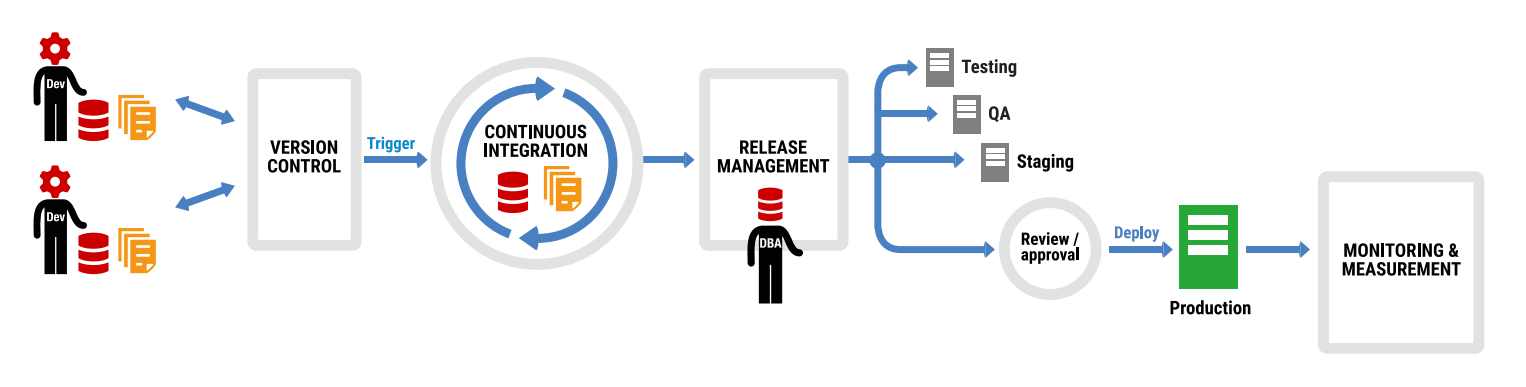
\includegraphics[width=14cm]{./IMAGENES/basededatos_1} 
		\caption{Incluyendo la base de datos en DevOps}
	\end{center}
\end{figure}

Como se puede ver, en lugar de que el desarrollo de la base de datos esté separado del de la aplicación y sea administrado al final por un equipo aislado, se convierte en una parte integral y natural de todo el proceso de desarrollo. Esta es una ventaja real para las empresas e instituciones donde, por lo general, la base de datos ha sido un cuello de botella. Debido a que la aplicación y la base de datos se desarrollan y prueban juntas, los errores o problemas potenciales se resaltan mucho antes en el proceso de desarrollo, evitando problemas cuando se implementan cambios. Compare esto con las conversaciones que he tenido con muchos DBA que deben revisar miles de líneas de script cuando se trata de implementar cambios en la base de datos. Eso puede llevar días, dependiendo de cuántos errores encuentren en el script. Al enviar cambios de la base de datos al control de origen de manera regular, puede introducir compilaciones y pruebas automatizadas para asegurarse de que todas esas pequeñas unidades de cambio se prueben y validen varias veces antes de que esté listo para implementar en su próximo entorno. Esto hace que las versiones sean más confiables y consuman menos tiempo, y también significa que puede responder a los cambios mucho más rápido. \cite{DevopsBD2}


%% ----------------------------------------------------------------------------------------------------------------------------------


%% ANÁLISIS ( APLICACIÓN ) ---------------------------------------------------------------------------------------------------

\section{Análisis}

EDITAR

%% ----------------------------------------------------------------------------------------------------------------------------------


%% CONCLUSIONES ---------------------------------------------------------------------------------------------------------------

\section{Conclusiones}

\begin{itemize}

\item Conclusion 1 : \\ A

\item Conclusion 2 : \\ B

\item Conclusion 3 : \\ C

\end{itemize}

%% ----------------------------------------------------------------------------------------------------------------------------------

%%  REFERENCIAS BIBLIOGRÁFICAS ------------------------------------------------------------------------------------------
	
	\newpage
	
	\bibliographystyle{apalike} 	%ESTILO
	\bibliography{BIBLIOGRAFIA}	 
	
	
\end{document}
